\section{Conclusion}
\subsection*{Discussion}
\begin{figure}
\centering
\fbox{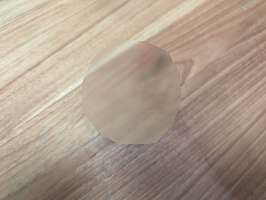
\includegraphics[width=0.8\linewidth]{../data/fullOutput2}}
\caption{PatchMatch fill output present on my project poster.}
\label{fig:blur}
\end{figure}

After running my PatchMatch algorithm on the apple dataset, I noticed that the output (\ref{fig:blur}) was very blurry. At first, I rationalized that the hole was too large (around $\frac 18$th the size of the image) and too round, causing the window size to be too large and the vote aggregation to include too many disparate vectors, resulting in a blurry outputted pixel. However, after reviewing my code I realized I was inputting the target image as a source as well, and so the blurriness from upscaling was being carried over between steps. After changing the code to remove the target from the sources, the output became much less blurry (\ref{fig:pmapple}).

Based on my experiments in this paper, I have come to the unfortunate conclusion that modern neural nets will outperform my handcrafted PatchMatch algorithm in the majority of situations. However, the silver lining is that in specific instances, such as the Spongebob dataset, my handcrafted algorithm will still produce visually better results.

\begin{figure}
\centering
\fbox{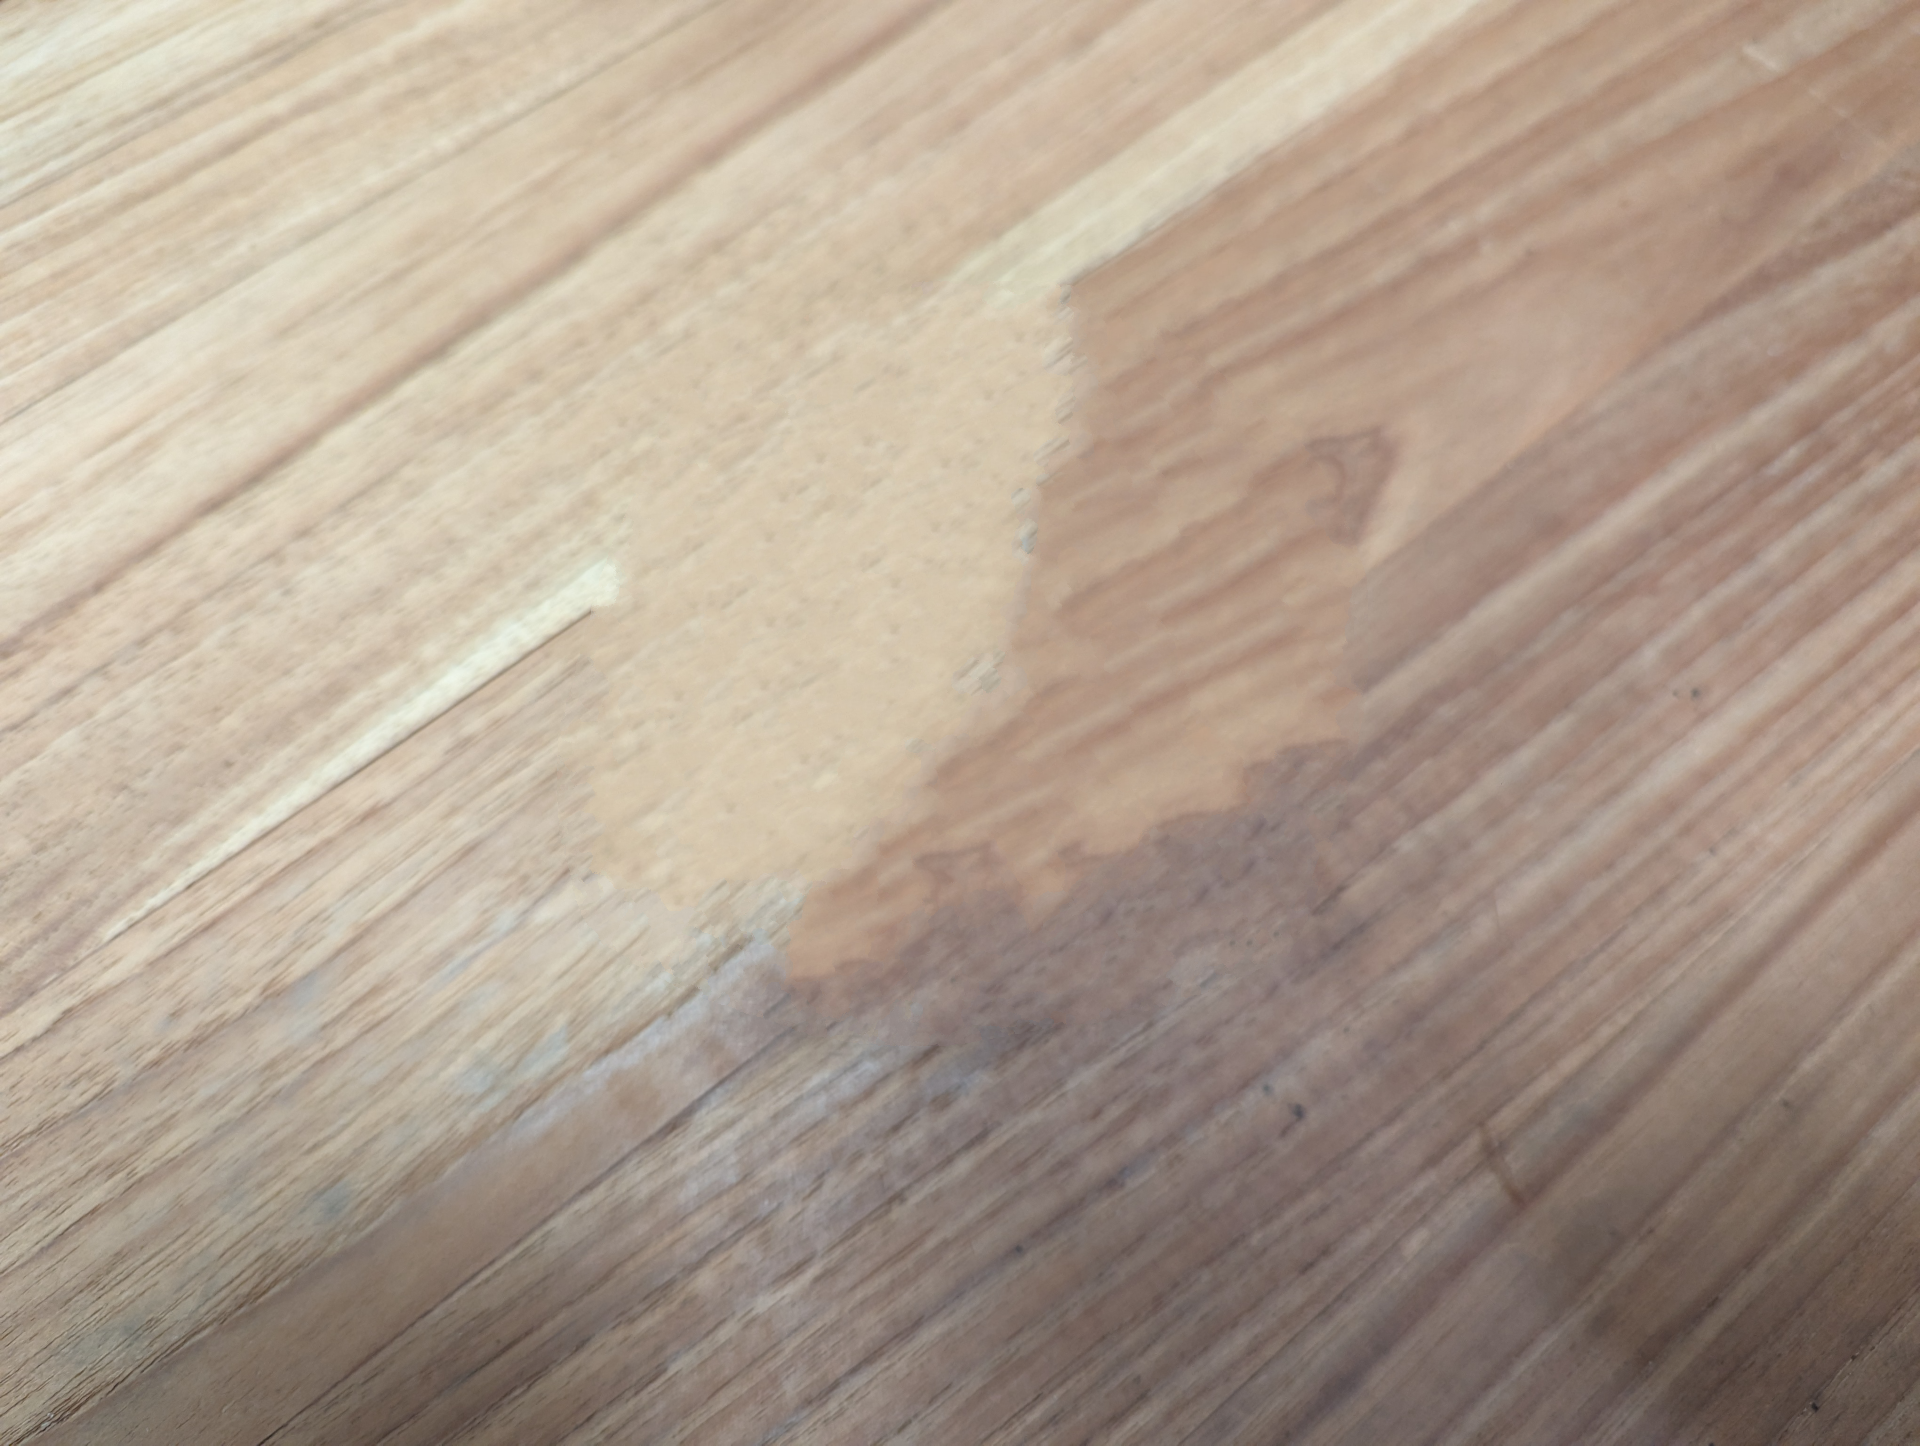
\includegraphics[width=0.8\linewidth]{../data/pixlr}}
\caption{Neural net hole fill present on my project poster.}
\label{fig:pixlr}
\end{figure}

Originally, the neural net I was using was one from pixlr.com, which did not produce very good results (\ref{fig:pixlr}). I found out about LaMa after the poster presentation while looking online to make sure that I was truly pitting my algorithm against the best that neural nets could offer. It was a bit shocking how much better it was able to perform on the apple dataset, but I'm glad that my PatchMatch algorithm could outperform LaMa on the Spongebob dataset. In both cases LaMa was much faster, though.

It seems that PatchMatch will still have a place when it comes to certain video applications like cartoons and movies, where the camera and lighting remain relatively stable between frames. As for Efros Leung, it seems like there is no longer a setting where it could be the best hole filling algorithm for the job.

\subsection*{Future work}
There are a few improvements to my PatchMatch algorithm that I will make in the future.

First is that I will probably migrate the code from Python to C++. I only coded in Python in the first place to be sure that any partners from this class would know the language. The switch to C++ should allow me to achieve a better runtime and also simplify the logic with my own data structures. I already mentioned that a doubly linked list would have been helpful, but my own image tensor data structure would have been helpful too, so that I could store my NNF and NND in the same data structure as the pixel values and more easily process edge cases.

A feature I wish to add is the ability to have different dimensions for the target and source images. In the PatchMatch paper, it is assumed that both will have the same dimensions, but from a mathematical standpoint, I do not think there is a reason why they should have to be. Another feature I wish to add is the ability to have holes in the source images. Similar to the feature of having different sized sources, this would make the algorithm compatible with more inputs.

One feature from the original paper that I probably will not include is the structure and feature guides that they allow users to draw. Since I have not created a GUI, it would be difficult to implement this, and it goes beyond the scope of what I want to do with this project.